\subsection{Cell Column Model}

\begin{supplementaryfigure}
    \centering
    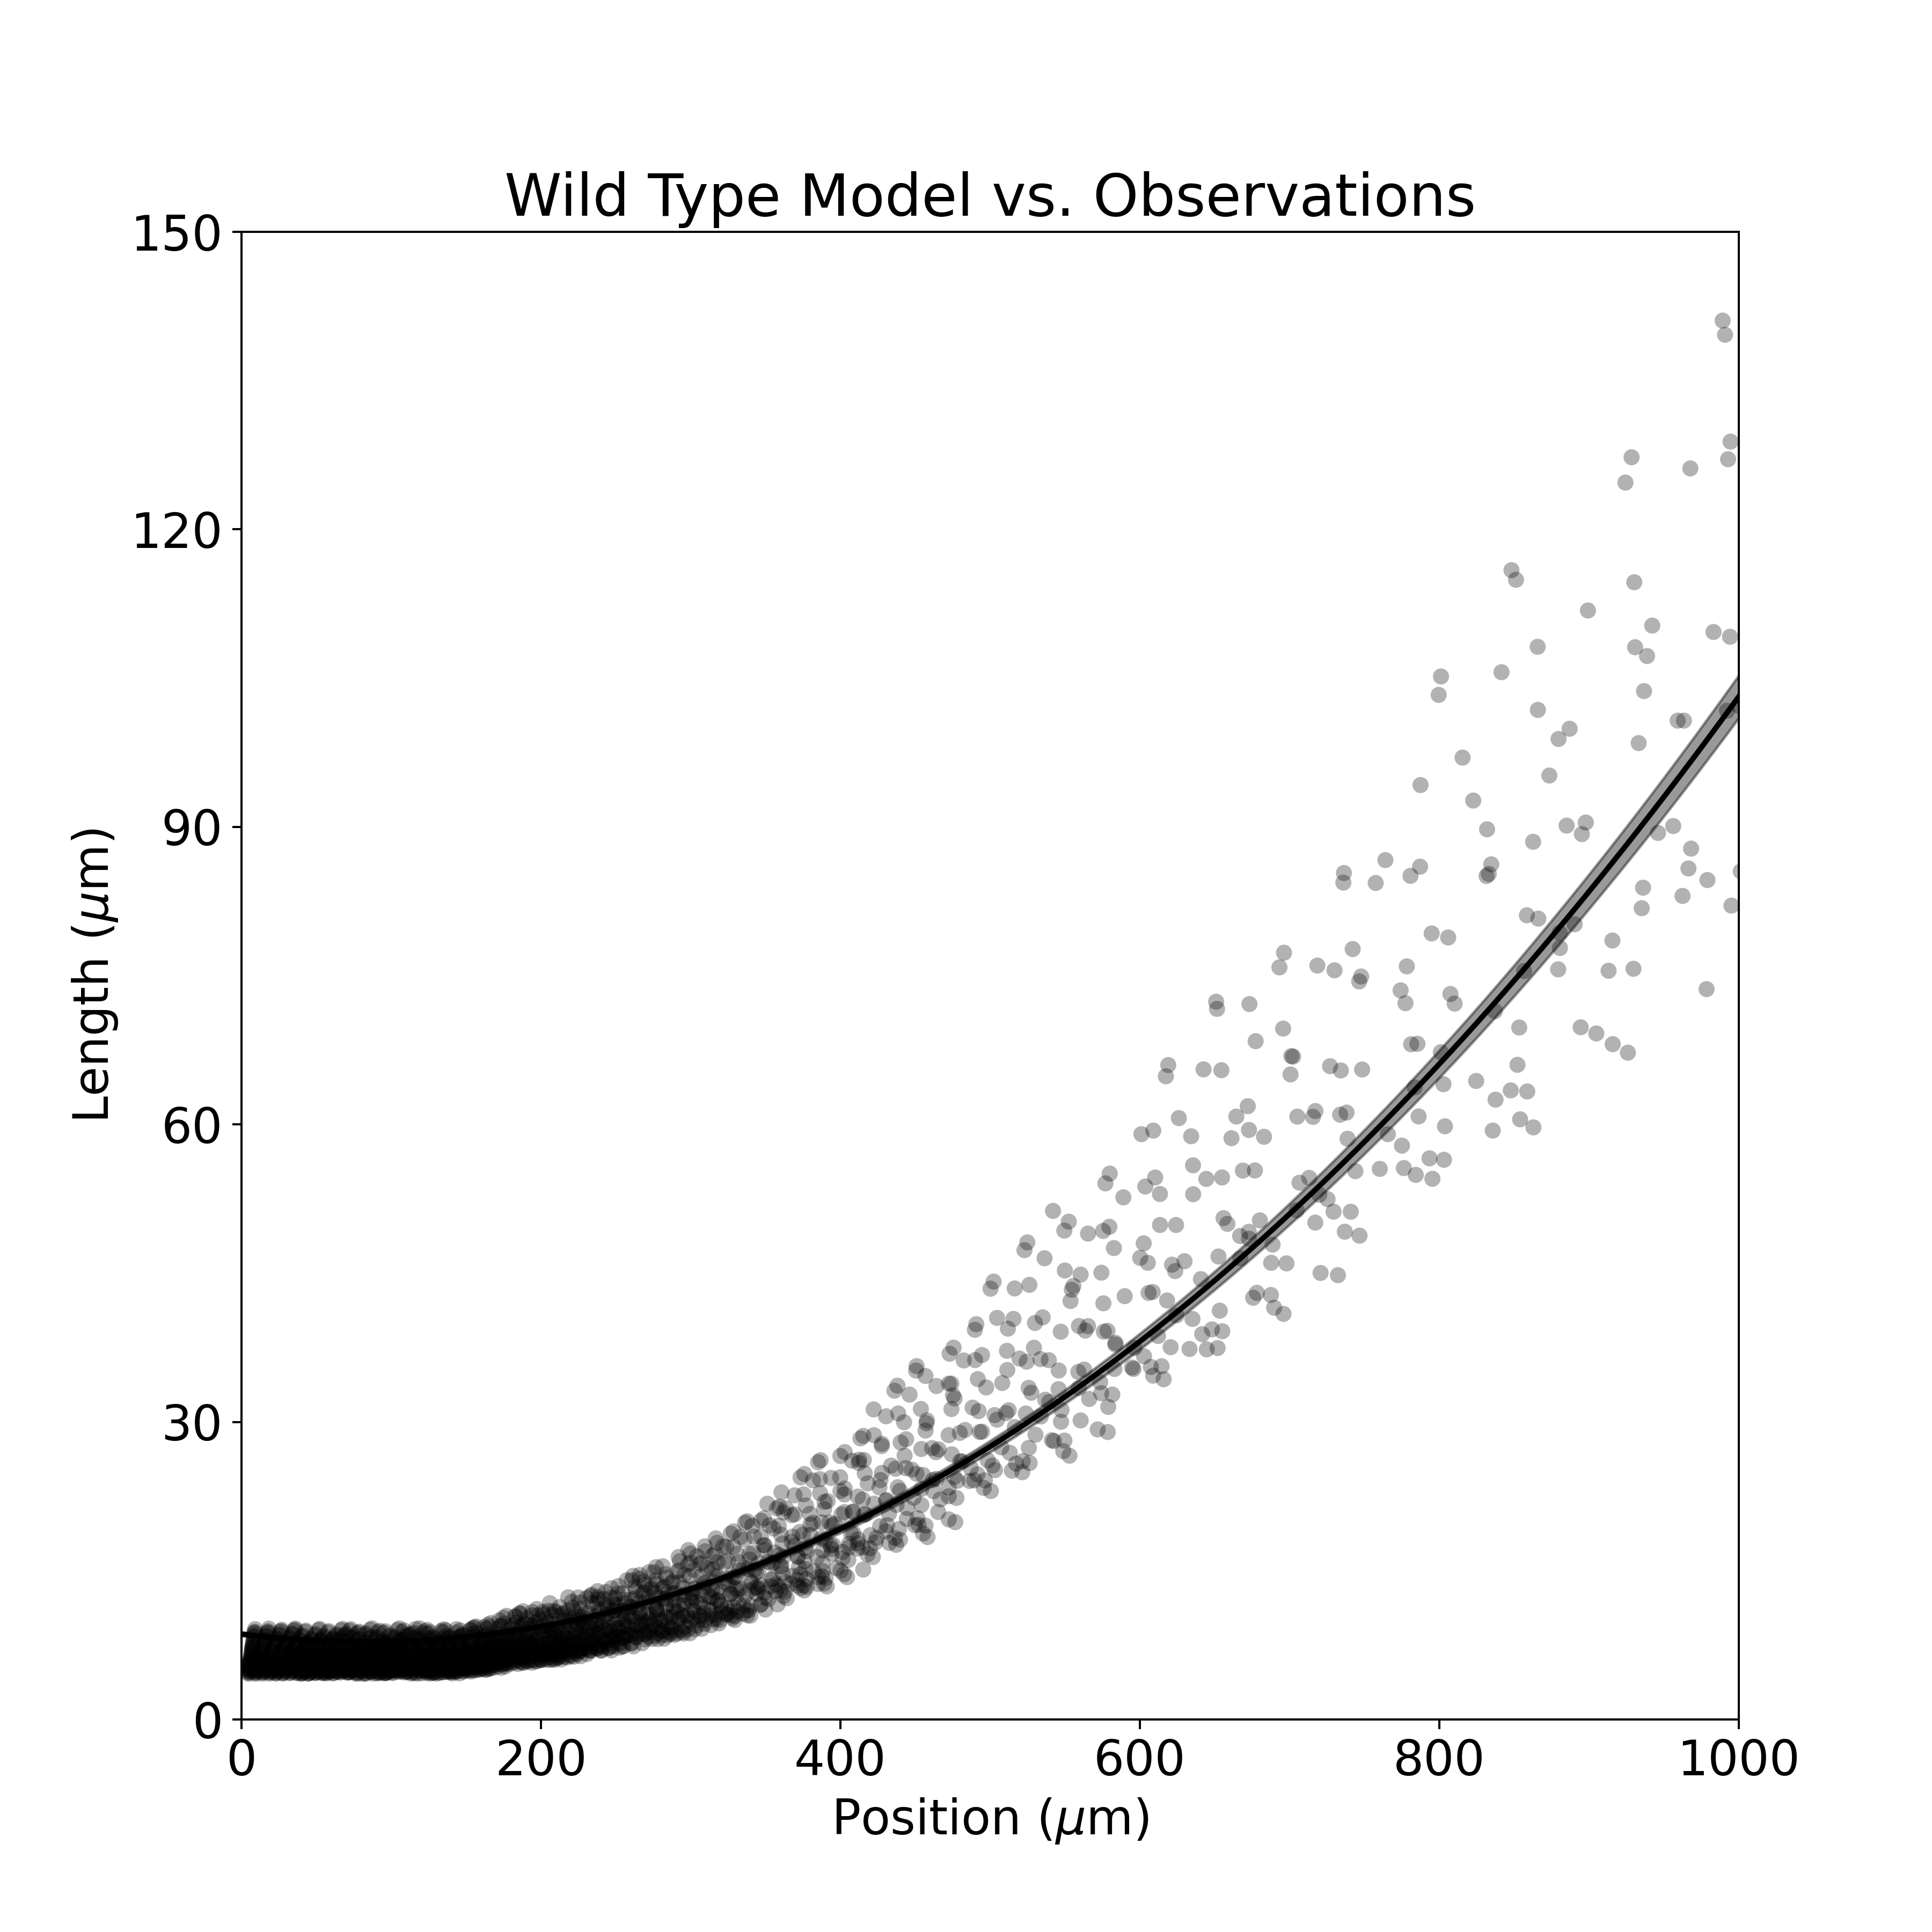
\includegraphics[width=13cm]{column-wild-type.png}
    \caption{Comparison of wild type cell column model with observations.}
    \label{sfig:column-wild-type}
\end{supplementaryfigure}

\begin{supplementaryfigure}
    \centering
    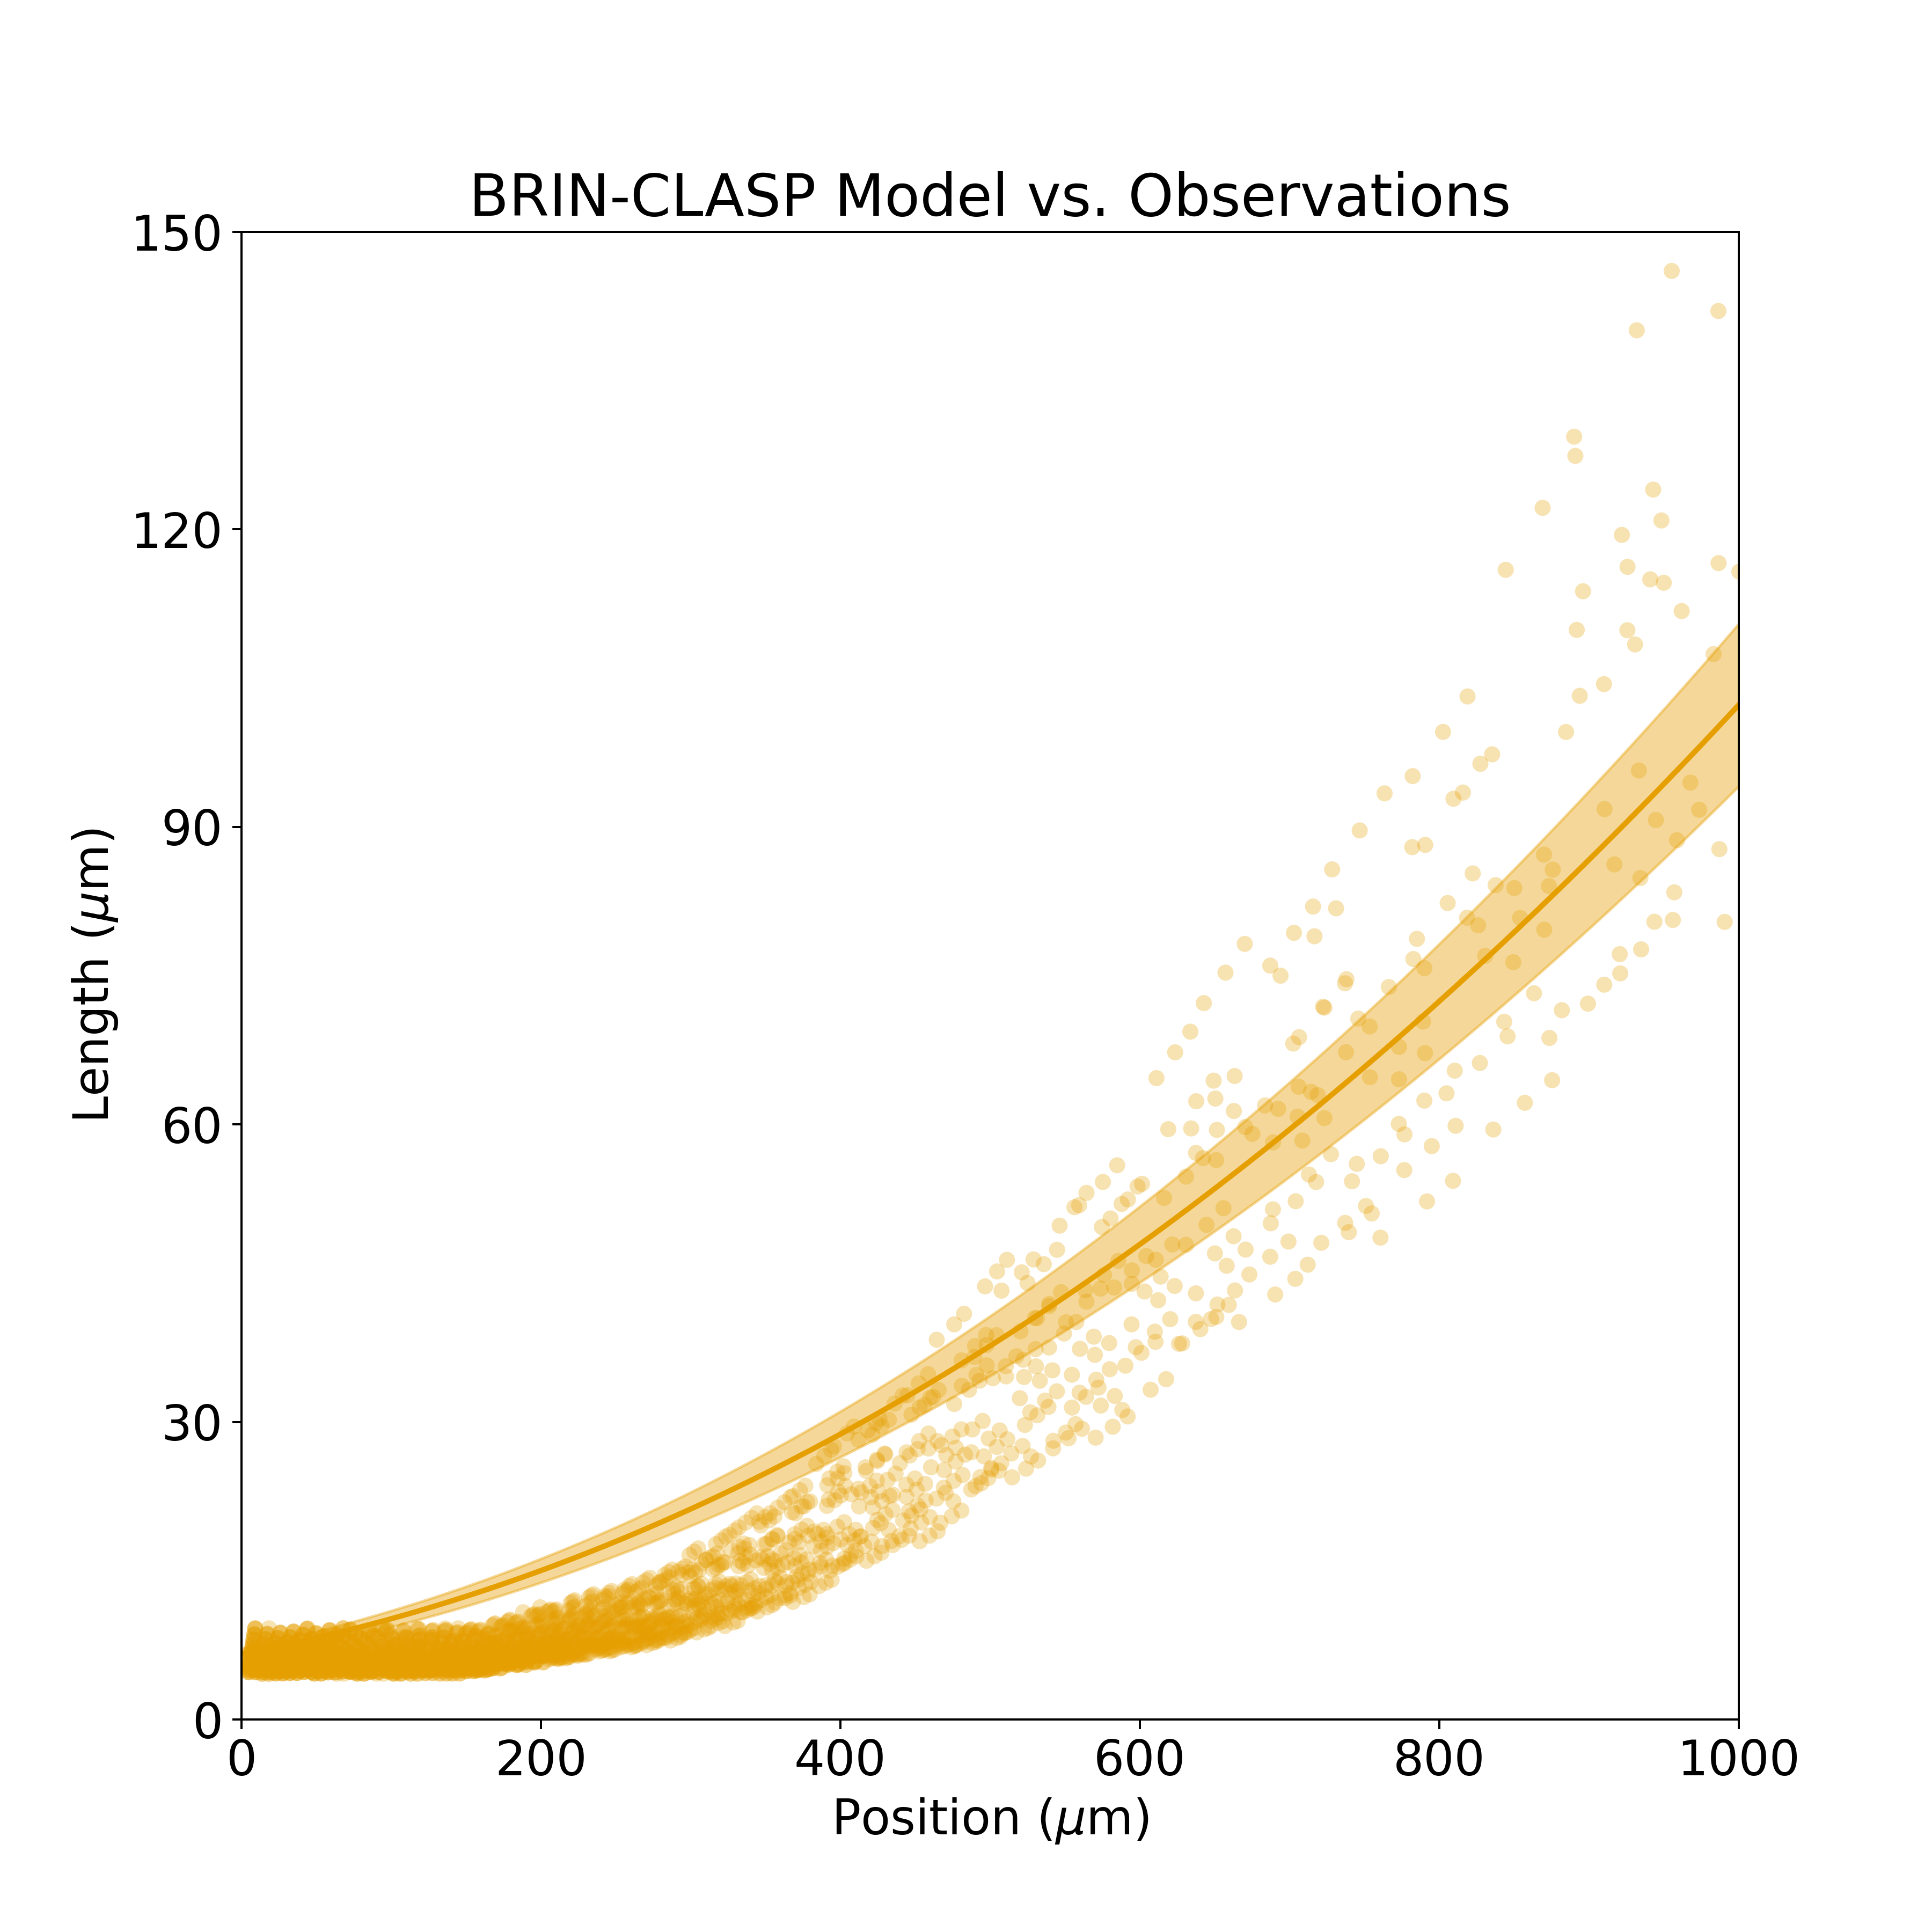
\includegraphics[width=13cm]{column-brin-clasp.png}
    \caption{Comparison of BRIN-CLASP cell column model with observations.}
    \label{sfig:column-brin-clasp}
\end{supplementaryfigure}

\begin{supplementaryfigure}
    \centering
    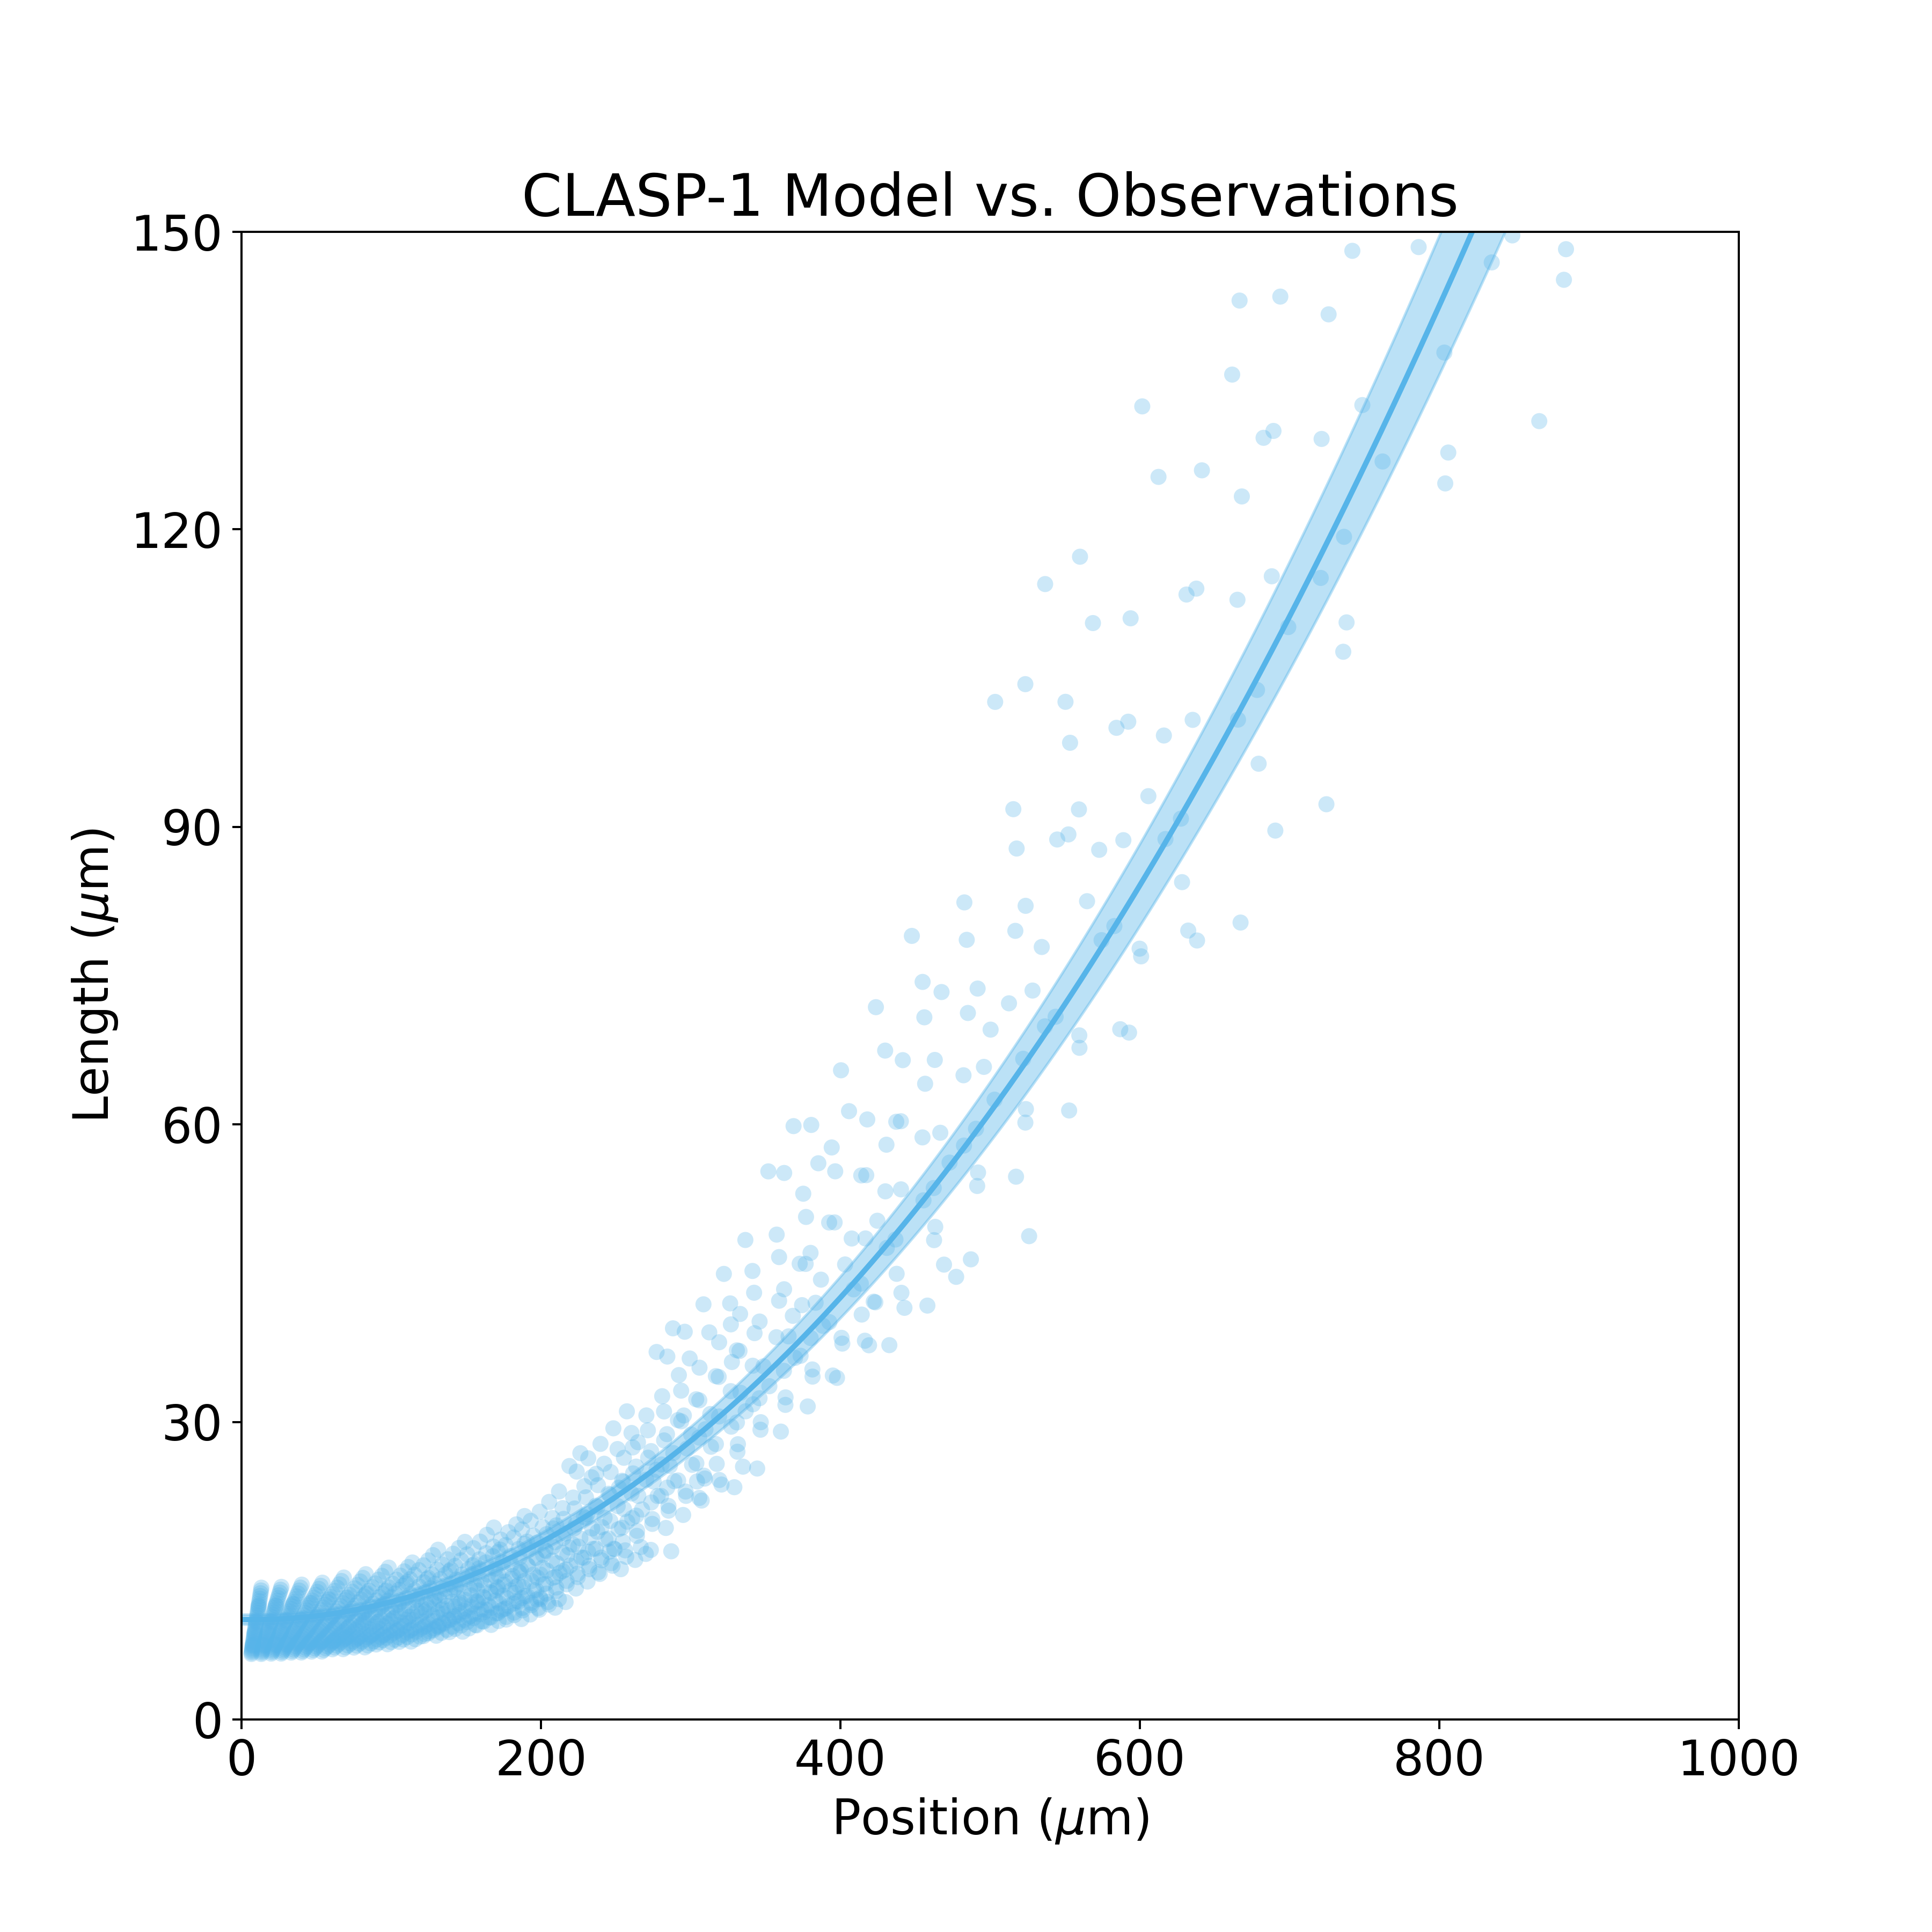
\includegraphics[width=13cm]{column-clasp-1.png}
    \caption{Comparison of CLASP-1 cell column model with observations.}
    \label{sfig:column-clasp-1}
\end{supplementaryfigure}

\begin{supplementaryfigure}
    \centering
    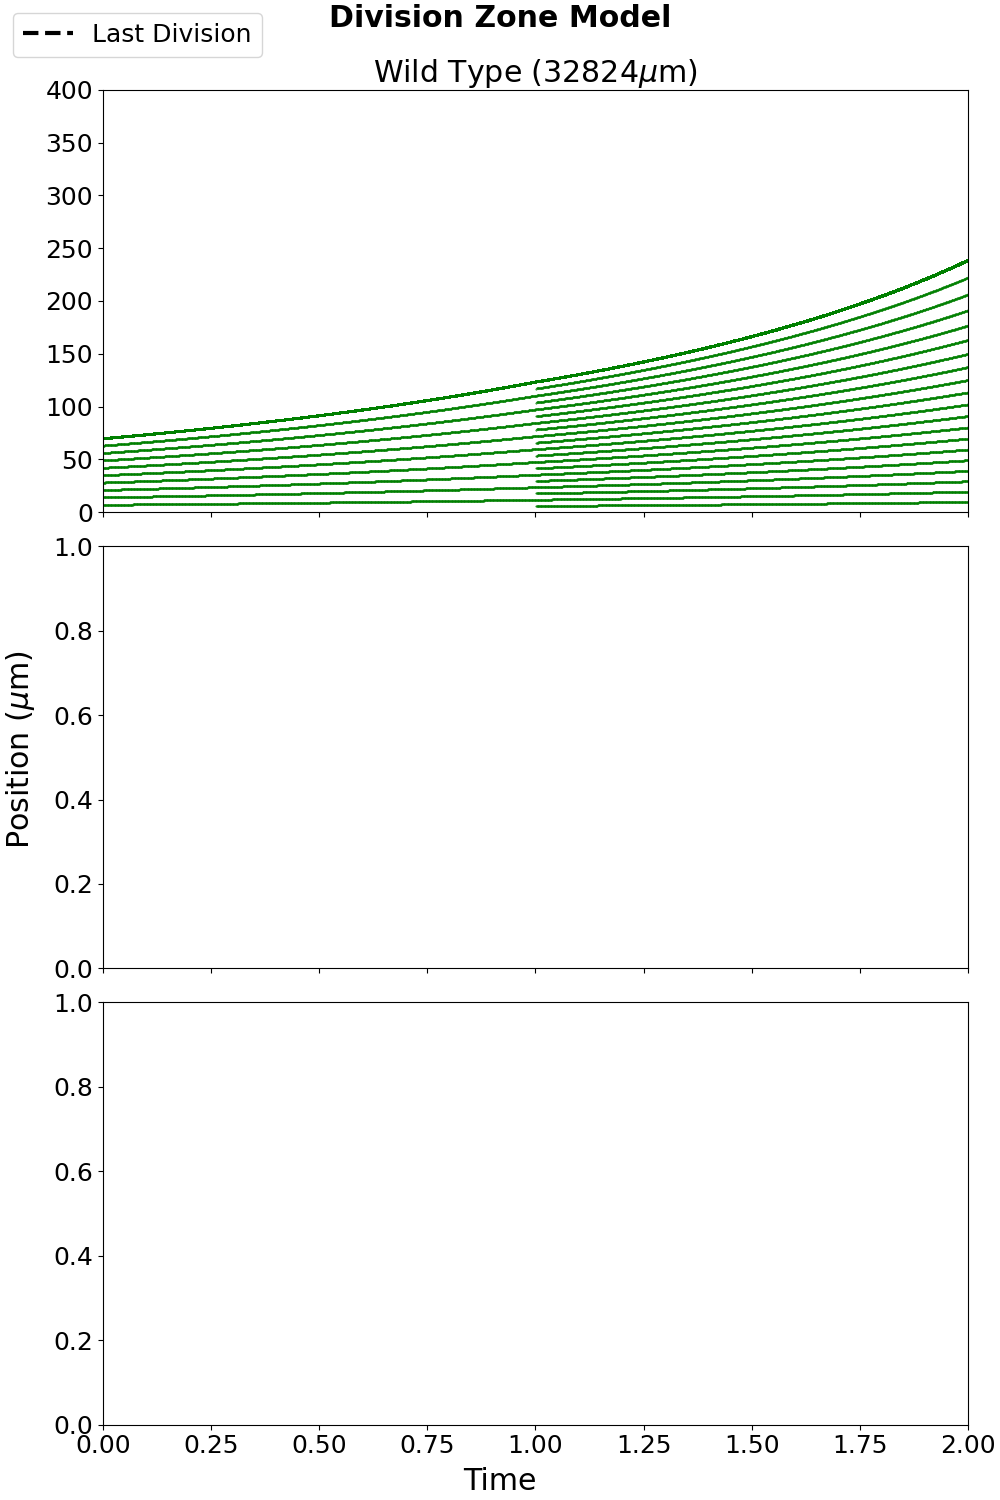
\includegraphics[width=13cm]{column-division-zone.png}
    \caption{A plot of the simulated cells in the division zone.}
    \label{sfig:column-division-zone}
\end{supplementaryfigure}

\begin{supplementaryfigure}
    \centering
    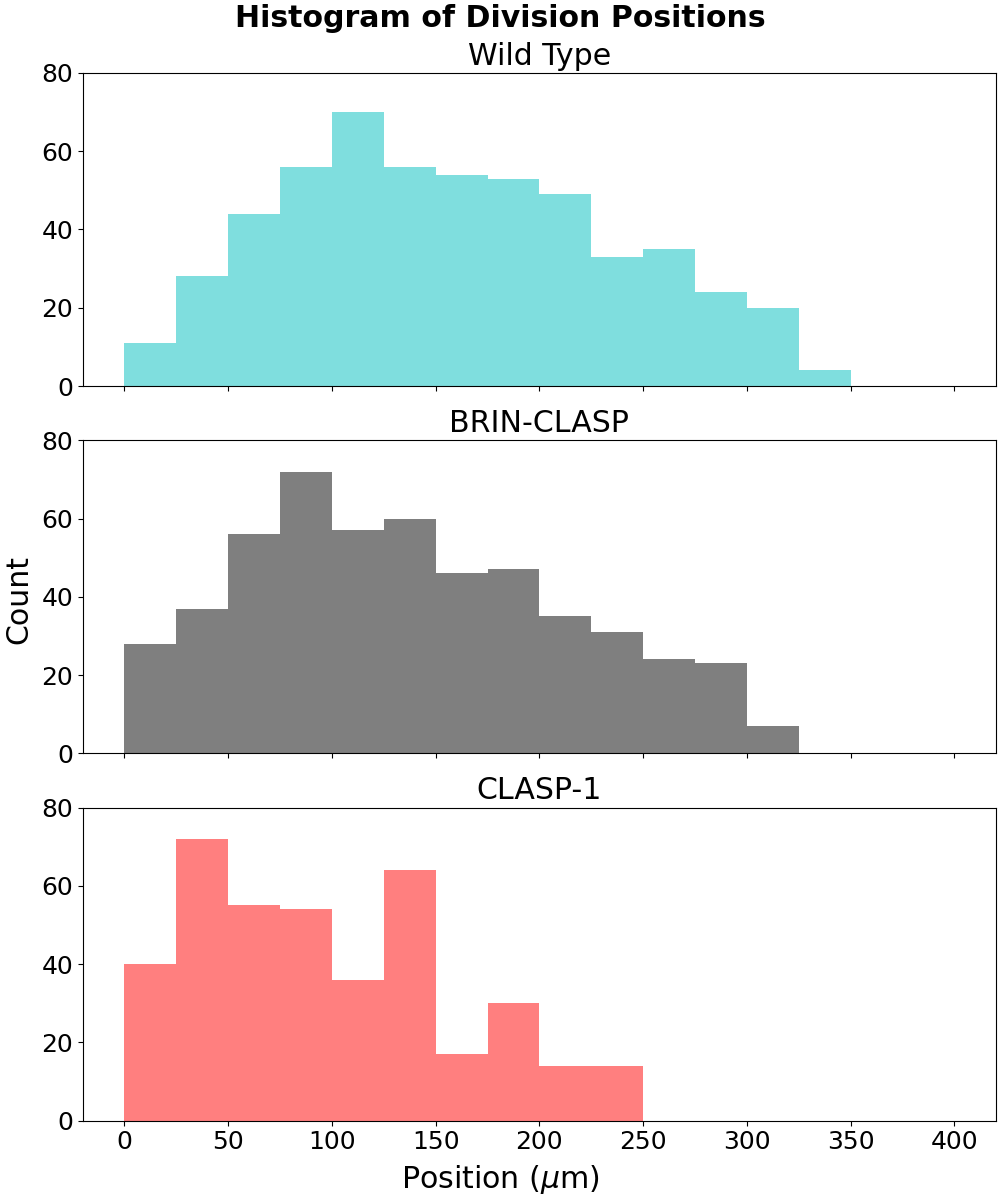
\includegraphics[width=13cm]{column-division-histogram.png}
    \caption{A histogram of division positions in each the two mutants and wild type.}
    \label{sfig:column-division-histogram}
\end{supplementaryfigure}
